\chapter{Characterization of the Soft Materials Behaviour} \label{ch:characterizationSoft}

\textbf{ \huge To-Do List}

Explain characterization process following a systematic approach:
\begin{itemize}
    \item In the introduction:
    \begin{itemize}
        \item[$\cross$] Mention the two performed mechanical tests and general parameters
        \item[$\cross$] Justify the reason why those tests were performed
        \item[$\cross$] List the soft materials analyzed
        \item[$\cross$] Describe how the specimens to test were extracted from the material sheets
        \item[$\cross$] Illustrate the specimens layout, recommended in the test standard, using my own SolidWorks drawing with dimensions
    \end{itemize}
    \item Tensile strength test:
    \begin{itemize}
        \item[$\cross$] Describe the test
        \item[$\cross$] List the parameters extracted
        \item[$\cross$] Describe the load-deformation curve
        \item[$\cross$] Compile in a table the deformation rate used for each material (this table can be placed instead in the section where the different datasets used to train the neural networks is mentioned).
        \item Describe the criteria used to decide how much to smooth the raw data
        \item Illustrate the obtained load-deformation curves
    \end{itemize} 
    \item Describe the stress relaxation test. Mention the parameters collected. Compile in a table the deformation to which each material was held during the test. Mention that initially the test duration was longer than the one being used for fitting the mathematical model.
    \item Describe now the pre-processing done to the collected raw data. Several conditions were established to decide how much to smooth the raw data.
    \item Present the obtained stress relaxation curves
\end{itemize}

Things to explain
\begin{itemize}
    \item Allowable attenuation of max value is 5 percent
    \item (Done) Consider cell resolution for limiting the amount of attenuation in the smoothing algorithm to the right amount. (The load cell used provides accurate measurements up to 1/500 of its capacity, i.e. for a load cell of 50 kN the smallest accurate measurement is 100N. All the soft materials implemented have load values in the range of 1 to 100 N. Therefore, using the accuracy parameters of the load cell as a guide is not possible.)
\end{itemize}

\section{Introduction}

In this chapter, the characterization process of seven rubber-based (elastomers) soft materials is presented. The selected soft materials are: ethylene polypropylene rubber (EPR), Fluorocarbon rubber (FR), nitrile rubber (NR), natural rubber with polyester (NatR),  polyethylene rubber (PR), silicone rubber (SR) and  off-the-shelf resistance bands of different thicknesses which are made of 100\% Natural Rubber (NatR100). Here in parentheses, the code names used for each material in future sections is presented.

In the first section, the mechanical properties of the selected elastomers is described and categorized as elastic and viscoelastic (time-dependent) properties. In the second section, the mechanical tests of tensile strength and stress relaxation, used for the characterization process, are described. The description of the algorithm implemented in Matlab to filter out the noise embedded in the experimental data is also included in this section. In the third section, a comparison analysis between the mechanical properties of the studied soft materials and the mechanical properties of the main tendon involved in the motion of the human knee joint (Patellar tendon), is presented.

\section{Mechanical Properties of Soft Materials} \label{mechprop}

The soft materials studied in this work belong to the thermoplastic elastomer family. Elastomers are created by mixing a thermoplastic material, such as natural or synthetic rubber, with other materials, such as carbon and sulfur. This process is called vulcanization which creates cross-linked structures inside the material. Since elastomers are based on rubber, the terms elastomer and rubber are often used interchangeably. Elastomers are known to have non-linear stress response, low stiffness and to achieve high deformation lengths. Some elastomers can fully recover their shape after stretched many times their length. They are also known to exhibit both elastic and viscoelastic properties. The latter means the stress response of elastomers is also time-dependent \cite{Bauman2008}. The main mechanical properties of elastomers are described in following paragraphs.
\subsection{Elasticity}
Elasticity, or elastic behaviour, refers to the ability of a material to be deformed up to a certain length and completely recover its shape and dimensions when the load deforming it is removed. Elasticity also refers to ability of a material to comply with the law of constant proportionality between the stress and the strain, described by Hooke's Law. However, elastomers are not purely elastic materials and tend to have a nonlinear stress-strain response, i.e. they do not obey Hooke's Law over the whole range of strains in the sense that the proportionality between the stress and the strain does not remain constant. This typical non-linear behaviour in the stress-strain curve of elastomers is illustrated in Figure \ref{fig:tensile}.

\begin{figure}[hb!]
    \centering
    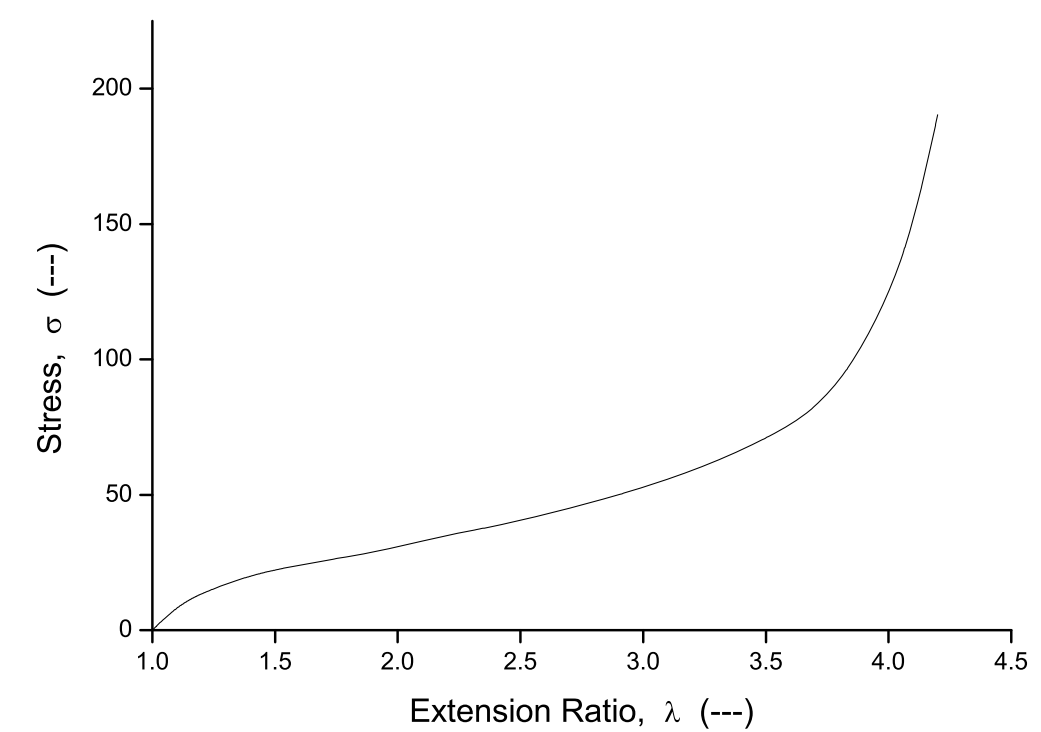
\includegraphics[width=0.7\textwidth]{TensileExample.png}
    \caption{Typical stress-strain curve of elastomers. \cite{Bauman2008}.}
    \label{fig:tensile}
\end{figure}

Elastomers are able to exhibit elastic behaviour up to a certain limiting load, known as the elastic limit. Beyond this limit the material is likely to undergo plastic or permanent deformation, this means the material will not recover its original shape completely. In some cases, the elastic limit is not easily visible from the stress-strain curve of a material and instead the proportional limit is used. The proportional limit defines the point in the stress-strain curve where the nonlinear response (change in the curve's slope) is first observed. Another way to delimit the elastic behaviour of a materials is using the yield strength which is defined as the maximum value on the curve or the first point in which an increase in strain occurs without an increase in strain \cite{ebewele2000}. These are some of the parameters that can be extracted from the tensile strength test and are useful to delimit the operating conditions of the materials.
\subsection{Viscoelasticity}
Viscoelasticity, is a property of some materials which are not purely elastic, do not fully obey Hooke's Law, nor purely viscous, do not fully obey Newton's Law, i.e. the stress is not proportional to the rate of change of the strain with time. In other words, the stress experienced by viscoelastic materials are dependent on both the amount and the speed of the strain applied to them. A purely elastic material is modelled, mechanically, as a spring; whereas a purely viscous material is modelled as a dashpot. By combining both of these elements it is possible to approximate the behaviour of a viscoelastic materials. These different combinations are known as the Linear Viscoelastic Models which will be described in latter sections. Finally, The time dependency of viscoelastic materials is appreciated in phenomenons such as creep, stress relaxation, hysteresis, the Mullin's Effect and in the Van der Waals forces.

Stress relaxation and creep are both time-dependent phenomenons observed in elastomers. On one hand, stress relaxation refers to the decrease over time of the stress experimented by a material when subjected to a constant strain (or deformation). On the other hand, creep refers to the increase over time of the material strain when subjected to a constant stress (or load). Understanding these phenomenons means understanding elastomers are composed of a network of molecular chains. Inside this network, entanglements form naturally. According to J. Bauman, stress relaxation is mainly caused by the slipping of these entanglements ultimately causing a loosening of force applied by the network of molecular chains. Stress relaxation and creep occur in both constant and cyclic deformations. Lastly, there are two mechanical tests designed to study these behaviours, from where it can be extracted the relaxation modulus and creep modulus of a material (\cite{oberg2016}). 

Hysteresis in a material is defined as the mechanical energy dissipated as heat when the material is undergoing deformations. This phenomenon is observed in a loading-unloading cycle, where the stress trajectory of the material while loading (extension) is different than the trajectory during unloading (retraction), as illustrated in Figure \ref{fig:hysteresis}. Hysteresis is mainly caused by internal friction of the molecular chain, also known as Van der Waals forces, in both elongation and contraction. Van der Waals forces are caused by the momentary bonding experienced between molecular chains that are close together. This constant making and breaking of bonds caused by deforming a material produces heat which ultimately becomes a mechanism to dissipate mechanical energy. This energy is represented as the enclosed area in Figure \ref{fig:hysteresis}. Stress relaxation and creep play a role in the amount of hysteresis experienced by a material in each consecutive loading-unloading cycle. The effect of hysteresis alone can be isolated by subjecting the elastomer to a conditioning process (preconditioning) in which it undergo several loading-unloading cycles until the stress response stops changing with every new cycle.

\begin{figure}[hb!]
    \centering
    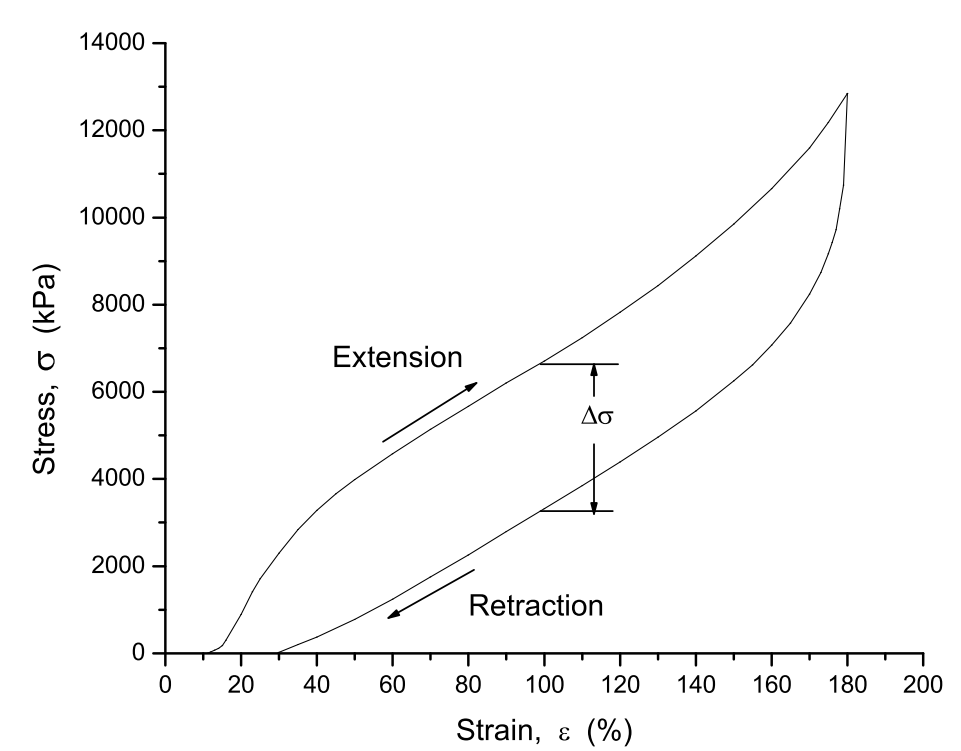
\includegraphics[width=0.7\textwidth]{HysteresisExample.png}
    \caption{Hysteresis in stress-strain curve. \cite{Bauman2008}.}
    \label{fig:hysteresis}
\end{figure}

The Mullin's effect is another important phenomenon to account for when studying the mechanical behaviour of elastomers. This effect refer to the breakage of tense molecular chains resulted from the manufacturing process of the material. Therefore, the very first time the material is subjected to deformations it exhibits a larger stress response in comparison to consecutive deformations. The latter is also referred to as a weakening of the material. This effect is more dramatic than the stress relaxation but can be easily avoided when preconditioning the material. Having defined the expected mechanical properties of elastomers, the mechanical tests of tensile strength and stress relaxation are described in the following section.

\section{Characterization Process}
In this section, the mechanical tests of tensile strength and stress relaxation, performed as part of the characterization process, are described. The tests are performed in an Instron 3369 Dual Column Testing System equipped with a 50 kN load cell, at room temperature (25 \degree C). The experimental data is expected to contain some noise due to the accuracy limitations of the available load cell. The algorithm implemented to filter this noise is described in SECTION . As previously mentioned, the elastomers selected for this research are: ethylene polypropylene rubber (EPR), Fluorocarbon rubber (FR), nitrile rubber (NR), natural rubber with polyester (NatR),  polyethylene rubber (PR), silicone rubber (SR) and  off-the-shelf resistance bands of different thicknesses which are made of 100\% Natural Rubber (NatR100). All the materials come in the form of a rectangular sheet. Laser cutting was used to extract individual specimens from each material sheet. In the Standard Test Method for Vulcanized Rubbers - Tension (ASTM D412), it is recommended to use five material specimens per test. Similarly, the recommended layout for the specimens, based on the thickness of the materials, is the Type C Dumbbell illustrated in Figure \ref{fig:specimenLayout} \cite{astmd412}.

\begin{figure}[hb!]
    \centering
    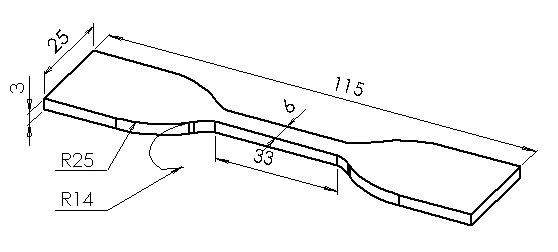
\includegraphics[width=0.6\textwidth]{SpecimenLayout.png}
    \caption{Specimen Type C Dumbbell Layout from the ASTM D412 \cite{astmd412}}
    \label{fig:specimenLayout}
\end{figure}

\subsection{Tensile Strength Test}

In a tensile strength test the material is loaded to failure at a certain deformation (strain) rate. The main purpose of this test is to extract the stress-strain curve of the material. From the stress-strain curve, the elastic properties of the material, such as stiffness, elastic modulus, ultimate strain, ultimate stress, elastic limit and yield strength, can be extracted. The stress-strain curve of elastomers (Figure \ref{fig:tensile}) has three main regions: the toe region, the elastic region, and the yield/failure region. In the toe region, the internal molecular chains of the material are misaligned, experiencing greater friction forces which greatly oppose to initial deformations. In contrast, when the molecular chains are aligned the friction forces decrease and the material deforms as a whole. The latter represent the elastic region, in which the slope of the curve (stiffness) is slightly smaller than in the toe-region. The elastic region of many materials exhibit a proportional or linear relationship between the stress and the strain. This is not the case for elastomers, where most of them exhibit a non-linear relationship. When the internal molecular chains have been elongated to its maximum length they demand higher forces to fail, this is observed as a peak in the load-elongation curve which also highlights the beginning of the yield/failure region \cite{Bauman2008}.

The tensile strength test performed in this work is in accordance with the Standard Test Method for Vulcanized Rubbers - Tension (ASTM D412) \cite{astmd412}. In here, it is recommended to elongate the material specimen until failure using a deformation rate of 500 mm/min, whenever possible. However, under certain circumstances where the previous deformation rate is not suitable, the test can be performed using the deformation rate of 250 mm/min. The latter was required for the silicon rubber, natural rubber and some resistance bands, where the gripper was not able to hold the material during the entirety of the test. In addition to the previous two deformation rates, a third one of 50 mm/min is used whenever possible. In summary, most of the materials are tested using at least two out of the three deformation rates of 50, 250 and 500 mm/min, to account for the deformation rate dependency, during the modelling stage, expected in the stress-strain curve of elastomers. The exact number of tests performed to each material is summarized in Table \ref{tbl:tensile_tests}.

\begin{table}[t]
    \centering
    \caption{Type and quantity of the different tensile strength tests performed. All the resistance bands are made of 100 \% Natural Rubber and are color coding depending on their stiffness.}
    \begin{tabular}{|C{0.3\textwidth}||C{0.2\textwidth}|C{0.1\textwidth}|C{0.1\textwidth}|C{0.1\textwidth}|}
    \hline 
    \multicolumn{5}{|c|}{Tensile Strength Datasets}\\
    \hline
    Type of Rubber & Thickness (mm) &   \multicolumn{3}{|c|}{ Deformation (mm/min)}\\
    \cline{3-5}
          &  & 50 & 250 & 500\\
    \hline
    Ethylene Polypropylene   &  1.5 & 16 & 0 & 5\\
    Fluorocarbon              &  1.5 & 9 & 8 & 5\\
    Natural with Polyester   &  1.5 & 10 & 5 & 0\\
    Nitrile                   &  1.5 & 7 & 7 & 5\\
    Silicone                  &  1.5 & 13 & 7 & 3\\
    Polyethylene              &  6 & 12 & 7 & 5\\
    \hline
    100\% Natural - Yellow  & 0.33, 0.42 & 1 & 6 & 1\\
    100\% Natural - Red  & 0.48, 0.52 & 0 & 8 & 0\\
    100\% Natural - Blue  & 0.64, 0.75 & 0 & 8 & 0\\
    100\% Natural - Green  & 0.97, 1.03 & 0 & 0 & 8\\
    100\% Natural - Black  & 1.17, 1.31 & 0 & 6 & 2\\
    100\% Natural - Orange  & 1.32, 1.49 & 0 & 5 & 0\\
    \hline
    \end{tabular}
    \label{tbl:tensile_tests}
\end{table}

One of the main parameters to extract from the obtained stress-strain curves is the elastic limit of each material. As previously mentioned in Section \ref{mechprop}, this parameter dictates the maximum amount of deformation a material can sustain without losing the ability to fully recover its original shape, i.e. its elasticity. Commonly, the proportional limit is used to approximate the location of the elastic limit, and by extension, the location of the elastic region. The proportional limit is the point in the curve where the proportionality between stress and stress becomes non-linear. It can be safely assumed that the elastic region of the material is located below this point. However, most elastomers do not have a clear elastic region due to their non-linear stress-strain curve, hence the proportional limit cannot be obtained. Under this circumstance, the elastic region of the material can be approximated using the yield strength of the material. The latter is defined as the first point in the curve where an increment in strain happens without and increment in the stress, hence the slope becomes zero or even negative \cite{astmd638}. In the scenario where the yield strength is difficult to extract, which is the case for most elastomers, the offset yield strength can be used as an alternative.

CONTINUE HERE(REMEMBER TO REVIEW PREVIOUS SECTION ABOUT PROPERTIES) - The calculation of the offset yield strength requires two parameters: the offset strain and the elastic modulus at a specific strain. In the literature, an offset strain of 2\% is recommended for plastics and elastomers (\cite{instron2019}). This recommendation is mainly to allow comparisons between different laboratories data and does not indicate a goodness of fit when approximating the elastic region or the yield point of a material. For the elastic modulus at a specified strain, the main recommendation is to select a portion at the beginning of the stress-strain curve in which a linear behaviour can be observed and apply a linear regression to this region to obtain the elastic modulus. In this work, the optimal strain range for the elastic modulus is obtained by trial and error. In summary, an offset strain of 2\% and an elastic modulus at 20\% strain were chosen to calculate the offset yield strength of all the materials which allowed us to approximate their elastic region and delimit their working conditions. 

Having defined these parameters, the first step to calculate the offset yield strength is to apply a linear regression to the first part of the curve (up to 20\% strain). The slope of this line represents the elastic modulus at the specified strain. The second step is to create a new line, starting from the specified 2\% offset strain, using the previously found elastic modulus as its slope. Finally, this line is projected up to the point in which it intersects the stress-strain curve. The stress and strain at this point represent the offset yield stress and the offset yield strain, respectively. Therefore, it is assume that beyond this point the material start undergoing plastic deformations. Similarly, it is assumed that the material is able to recover its original shape for all deformations found bellow the offset yield strain. Summarizing, the offset yield strength is illustrated in Figures \ref{fig:EPR} to \ref{fig:Nat100R} along with the initial part of the stress-strain curves of the studied materials for all the performed tensile strength tests. 
Furthermore, the elastic properties extracted from the stress-strain curves are reported in Table FILL.

\newpage
%The correct factor to fit to figures in the same line is 0.49
\begin{figure}[H]
    \centering
    \begin{subfigure}[b]{0.49\textwidth}
        \centering
        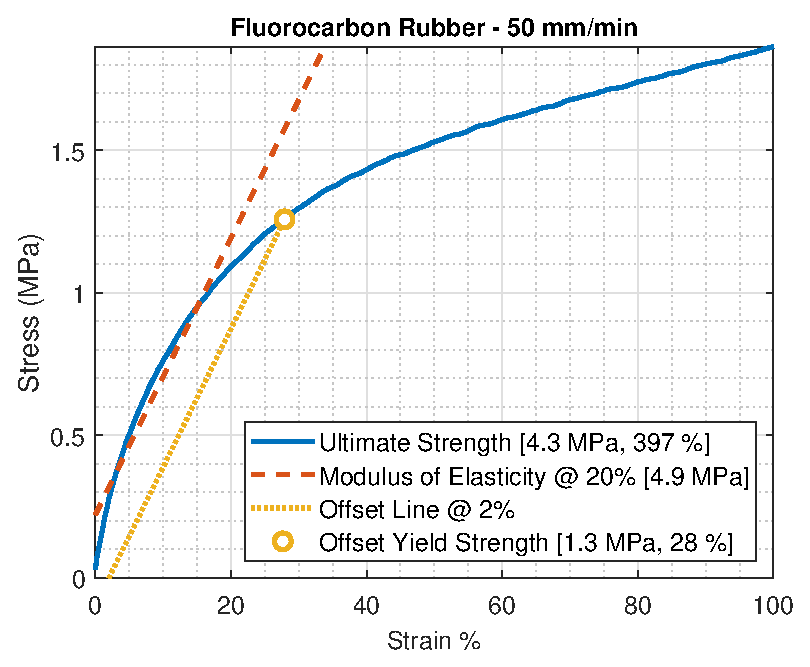
\includegraphics[width=\textwidth]{FR_disR50.eps}
        \caption{Caption}
        \label{fig:FR50}
    \end{subfigure}
    \hfill
    \begin{subfigure}[b]{0.49\textwidth}
        \centering
        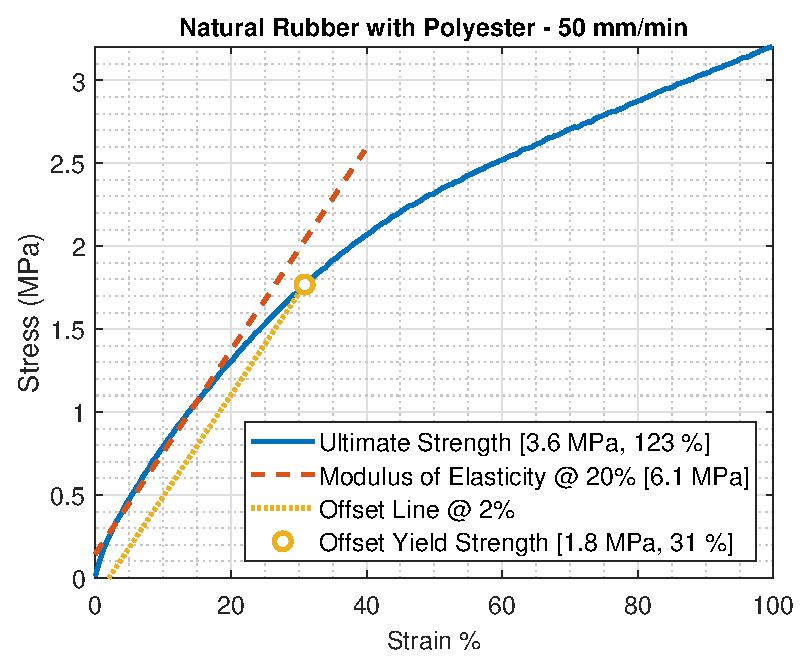
\includegraphics[width=\textwidth]{NatR_disR50.eps}
        \caption{Caption}
        \label{fig:FR250}
    \end{subfigure}
    \hfill
    \begin{subfigure}[b]{0.49\textwidth}
        \centering
        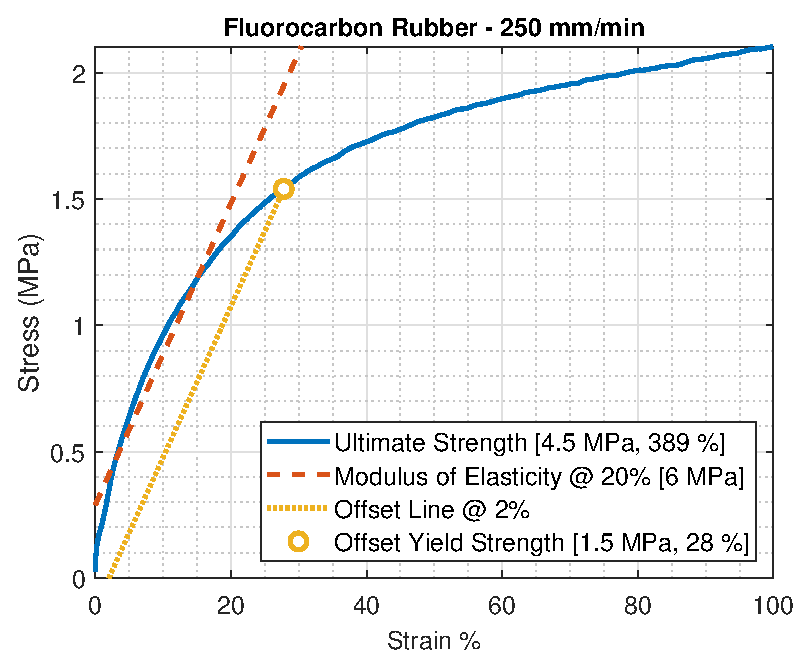
\includegraphics[width=\textwidth]{FR_disR250.eps}
        \caption{Caption}
        \label{fig:FR500}
    \end{subfigure}
    \hfill
    \begin{subfigure}[b]{0.49\textwidth}
        \centering
        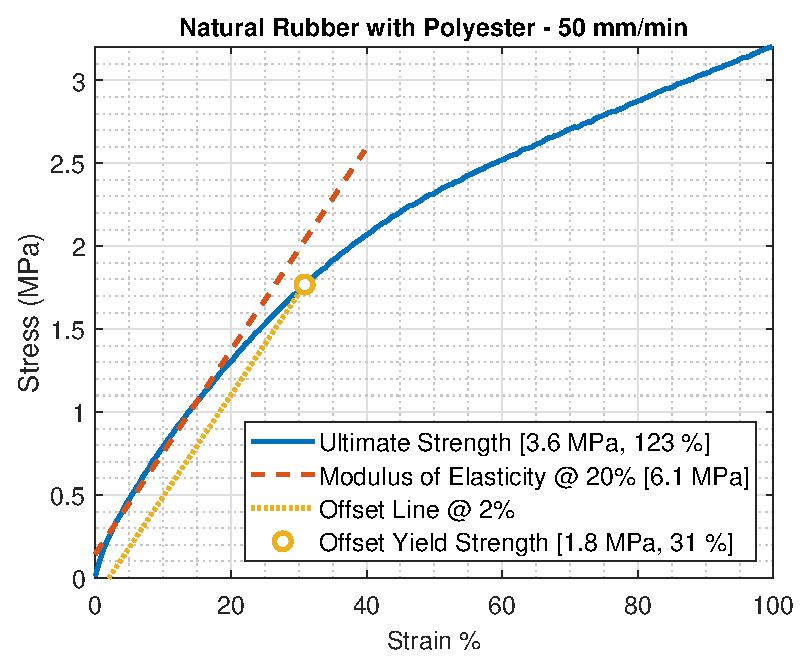
\includegraphics[width=\textwidth]{NatR_disR50.eps}
        \caption{Caption}
        \label{fig:NatR50}
    \end{subfigure}
    \hfill
    \begin{subfigure}[b]{0.49\textwidth}
        \centering
        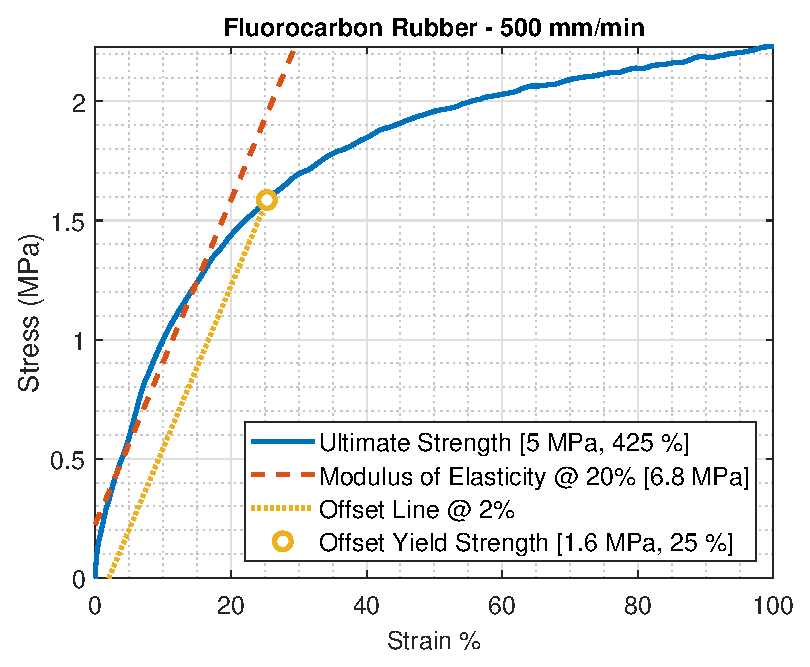
\includegraphics[width=\textwidth]{FR_disR500.eps}
        \caption{Caption}
        \label{fig:NatR250}
    \end{subfigure}
    \hfill
    \begin{subfigure}[b]{0.49\textwidth}
        \centering
        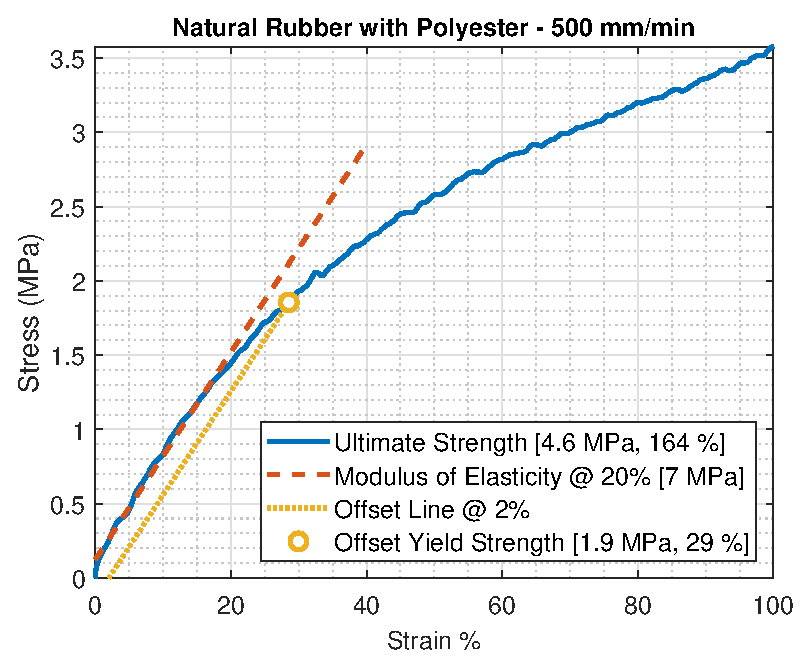
\includegraphics[width=\textwidth]{NatR_disR500.eps}
        \caption{Caption}
        \label{fig:NatR500}
    \end{subfigure}
    \caption{Caption for main figure}
    \label{fig:FRandNatR}
\end{figure}

\begin{figure}[H]
    \centering
    \begin{subfigure}[b]{0.49\textwidth}
        \centering
        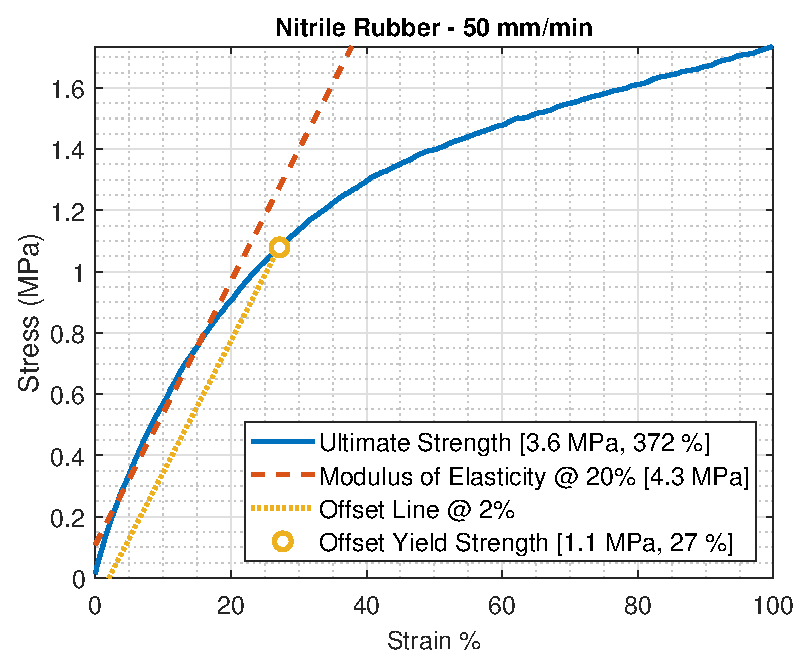
\includegraphics[width=\textwidth]{NR_disR50.eps}
        \caption{Caption}
        \label{fig:NR50}
    \end{subfigure}
    \hfill
    \begin{subfigure}[b]{0.49\textwidth}
        \centering
        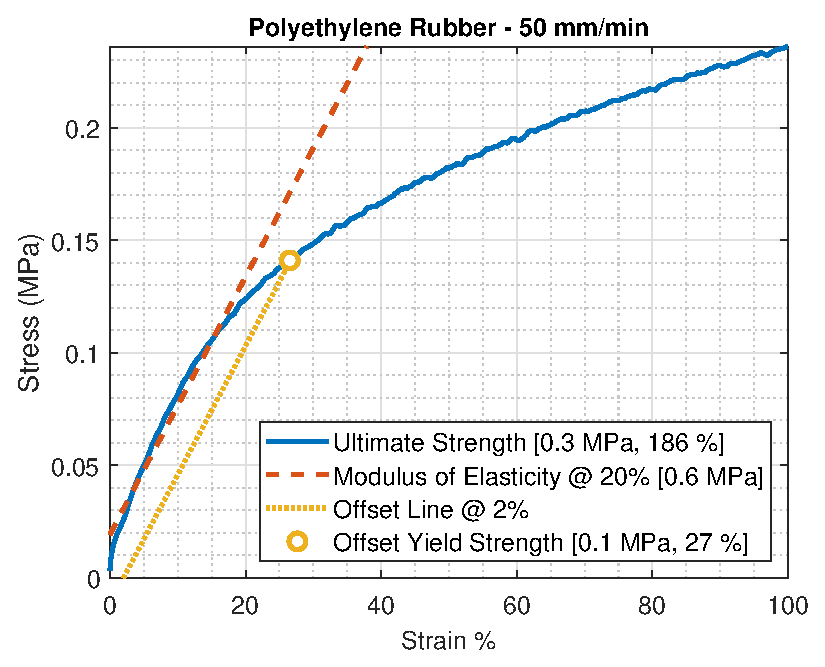
\includegraphics[width=\textwidth]{PR_disR50.eps}
        \caption{Caption}
        \label{fig:NR250}
    \end{subfigure}
    \begin{subfigure}[b]{0.49\textwidth}
        \centering
        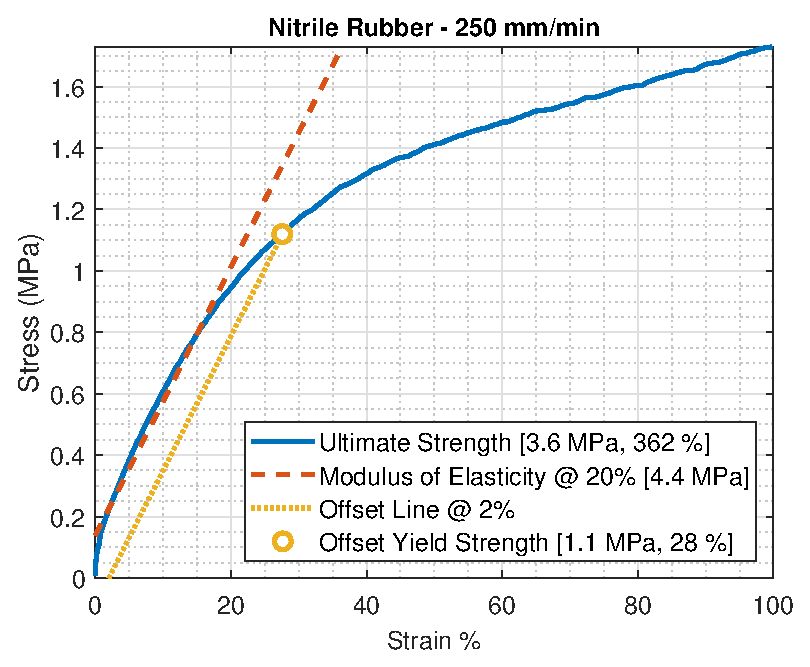
\includegraphics[width=\textwidth]{NR_disR250.eps}
        \caption{Caption}
        \label{fig:NR500}
    \end{subfigure}
    \hfill
    \begin{subfigure}[b]{0.49\textwidth}
        \centering
        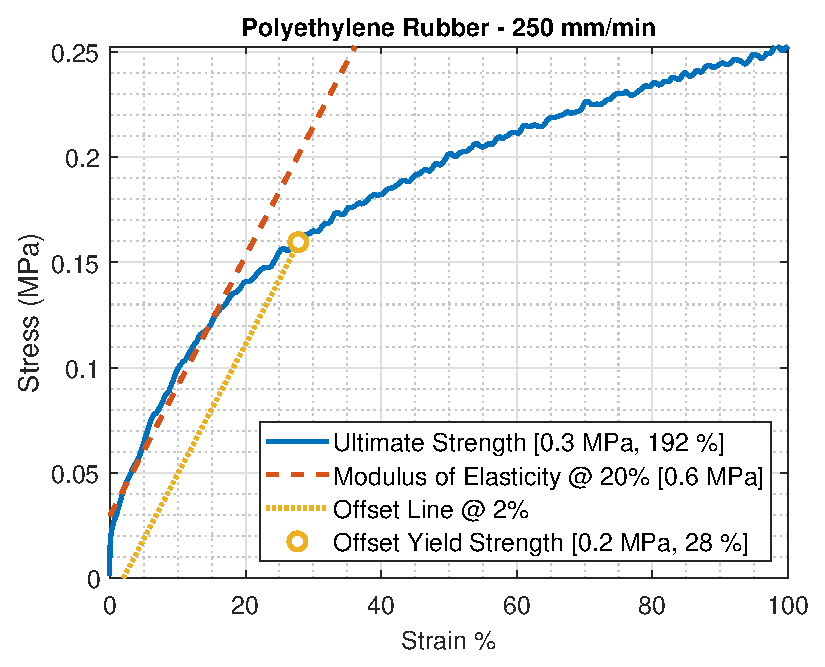
\includegraphics[width=\textwidth]{PR_disR250.eps}
        \caption{Caption}
        \label{fig:PR50}
    \end{subfigure}
    \hfill
    \begin{subfigure}[b]{0.49\textwidth}
        \centering
        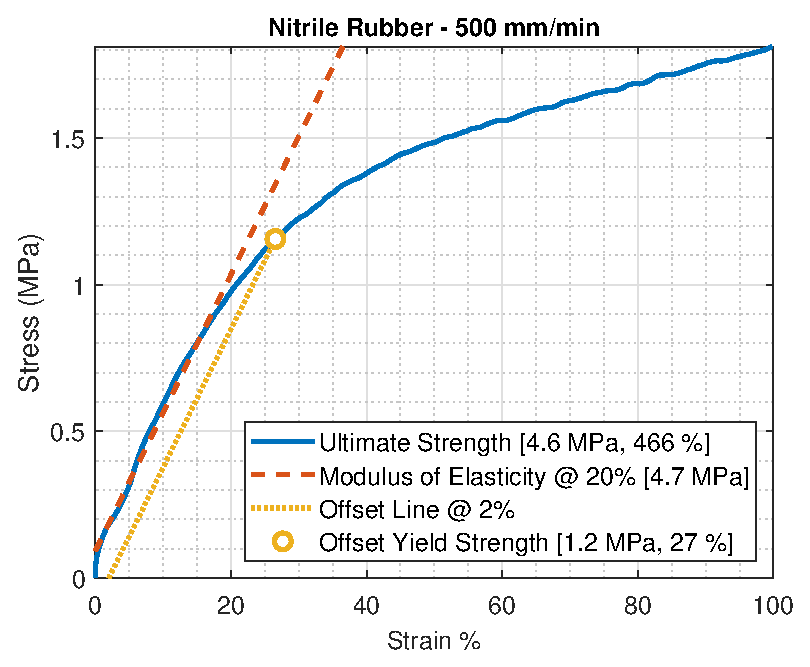
\includegraphics[width=\textwidth]{NR_disR500.eps}
        \caption{Caption}
        \label{fig:PR250}
    \end{subfigure}
    \hfill
    \begin{subfigure}[b]{0.49\textwidth}
        \centering
        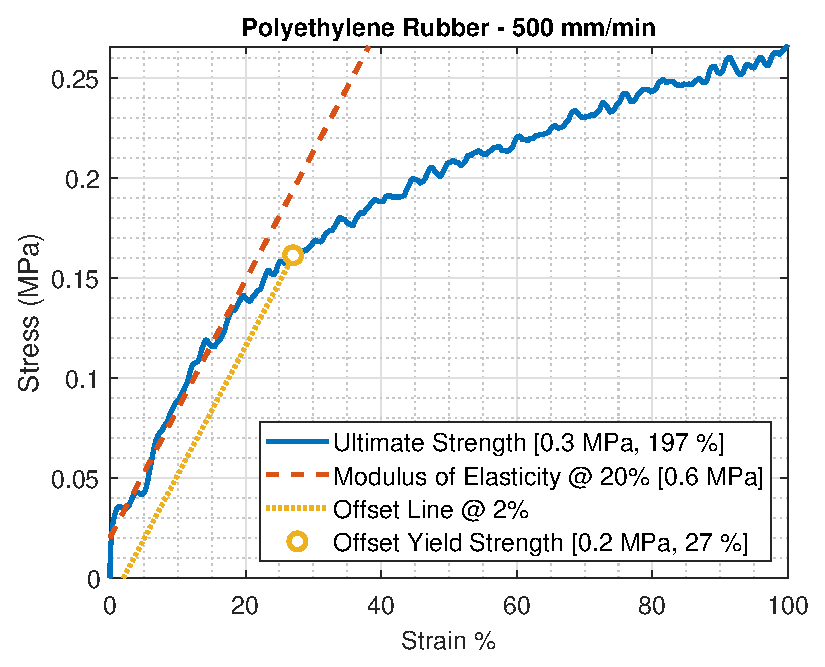
\includegraphics[width=\textwidth]{PR_disR500.eps}
        \caption{Caption}
        \label{fig:PR500}
    \end{subfigure}
    \caption{Caption for main figure}
    \label{fig:NR}
\end{figure}

\begin{figure}[H]
    \centering
    \begin{subfigure}[b]{0.49\textwidth}
        \centering
        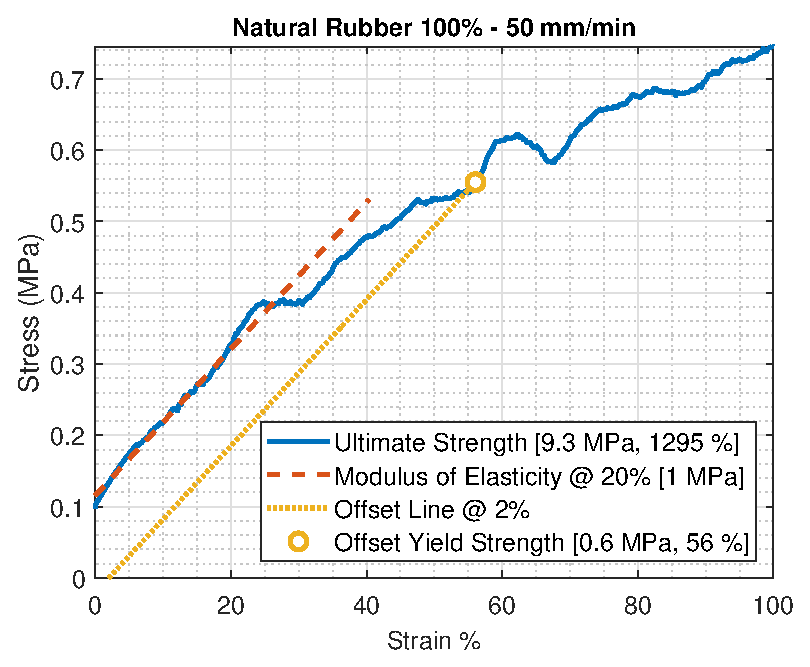
\includegraphics[width=\textwidth]{Nat100R_disR50.eps}
        \caption{Caption}
        \label{fig:Nat100R50}
    \end{subfigure}
    \hfill
    \begin{subfigure}[b]{0.49\textwidth}
        \centering
        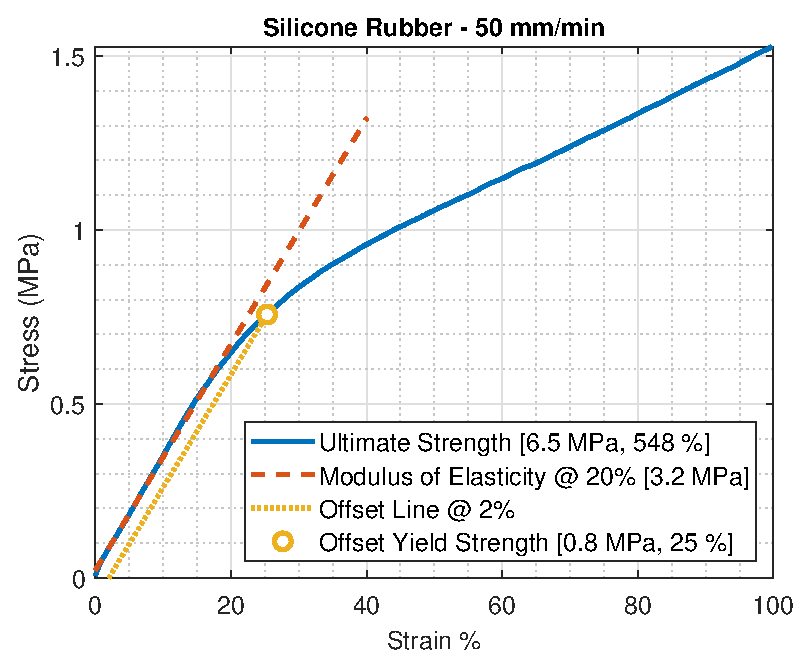
\includegraphics[width=\textwidth]{SR_disR50.eps}
        \caption{Caption}
        \label{fig:SR50}
    \end{subfigure}
    \hfill
    \begin{subfigure}[b]{0.49\textwidth}
        \centering
        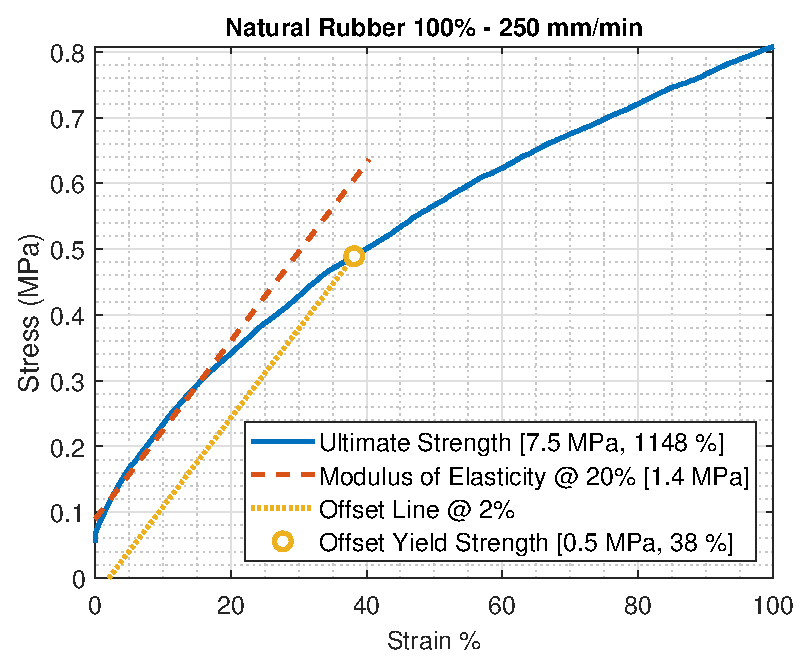
\includegraphics[width=\textwidth]{Nat100R_disR250.eps}
        \caption{Caption}
        \label{fig:Nat100R250}
    \end{subfigure}
    \hfill
    \begin{subfigure}[b]{0.49\textwidth}
        \centering
        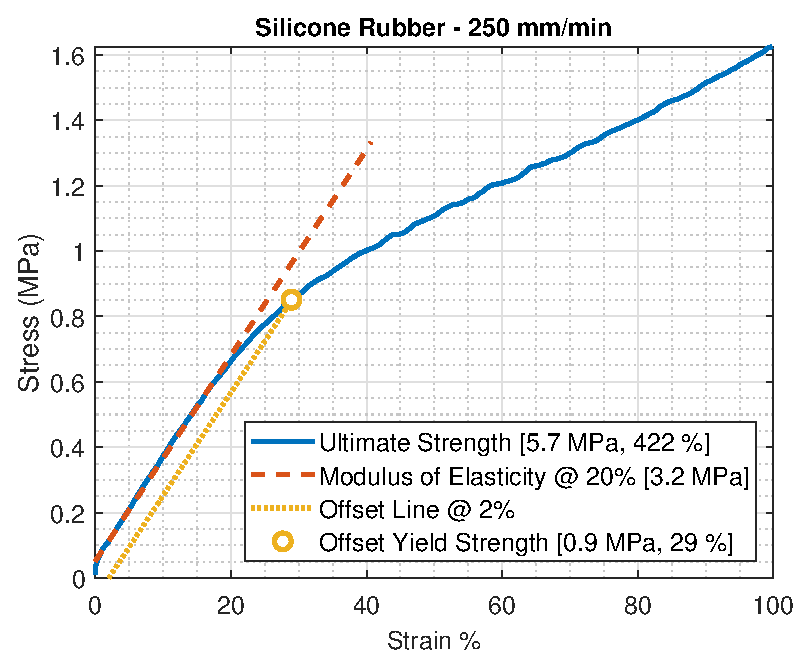
\includegraphics[width=\textwidth]{SR_disR250.eps}
        \caption{Caption}
        \label{fig:SR250}
    \end{subfigure}
    \hfill
    \begin{subfigure}[b]{0.49\textwidth}
        \centering
        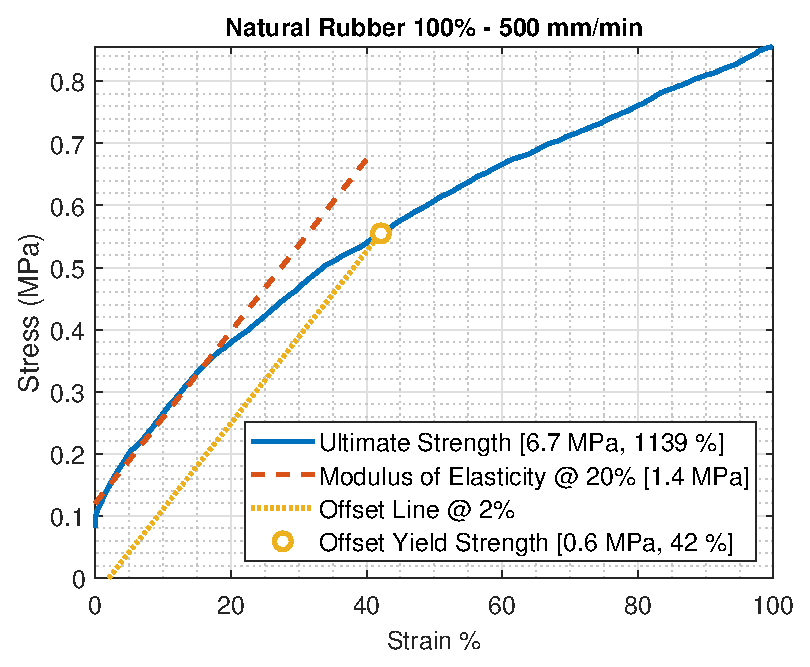
\includegraphics[width=\textwidth]{Nat100R_disR500.eps}
        \caption{Caption}
        \label{fig:Nat100R500}
    \end{subfigure}
    \hspace*{\fill}
    \caption{Caption for main figure}
    \label{fig:Nat100R}
\end{figure}

\begin{figure}[H]
    \centering
    \begin{subfigure}[b]{0.49\textwidth}
        \centering
        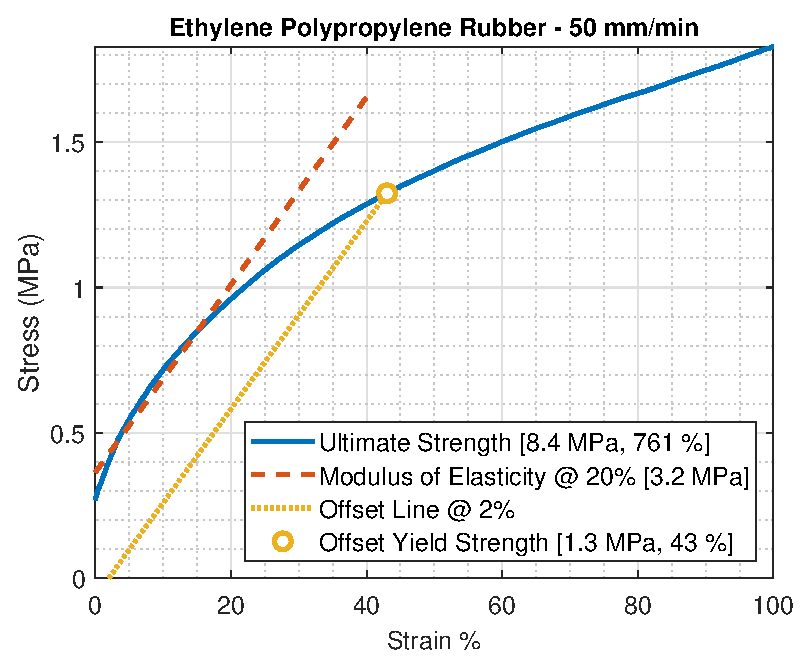
\includegraphics[width=\textwidth]{EPR_disR50.eps}
        \caption{Caption}
        \label{fig:EPR50}
    \end{subfigure}
    \hfill
    \begin{subfigure}[b]{0.49\textwidth}
        \centering
        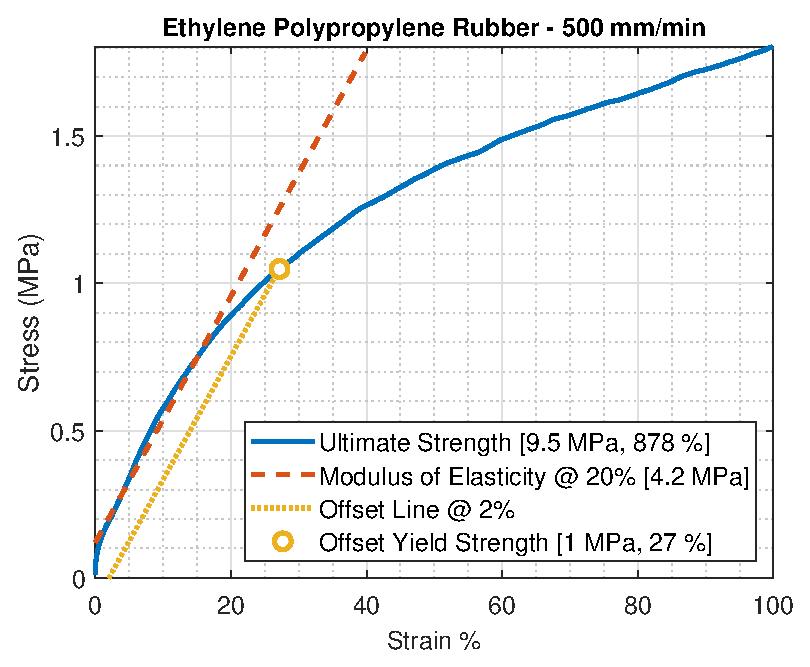
\includegraphics[width=\textwidth]{EPR_disR500.eps}
        \caption{Caption}
        \label{fig:EPR500}
    \end{subfigure}
    \caption{Caption for main figure}
    \label{fig:EPR}
\end{figure}

%Specimen Length used in the file Materials Properties has to be updated to 33 instead of 25
\begin{table}[ht!]
    \centering
    \begin{tabular}{c|c}
         &  \\
         & 
    \end{tabular}
    \caption{Caption}
    \label{tab:my_label}
\end{table}

crystallization of some materials

CRITICAL - The strain-stress curve for elastomers does not have a toe and elastic region. The effects are different and must be explained before describing the mechanical tests. Everything is summarized in Bauman's paper. More reading on the stress relaxation part is a must because I initially used the elastic region as a way to avoid plastic deformation. This can be better justified by the need of avoiding high strains to prevent chain ruptures. The first cycle of stress relaxation is the most important. More literature is required to support this. Also, crystallization explains the steep increase (stiffening) at the end of the curve in some of the rubbers I have. This chapter needs a rewriting. Moreover, plots with toe and elastic regions are no longer needed. Instead, plots showing the data from different strain rates of the same material are more suitable. The idea of training a neural network to predict the stiffness in real time is still viable. Van der Waals effects are important.

\subsection{Stress Relaxation Test}

The stress relaxation test allows the extraction of the viscoelastic (time-dependant) properties of the materials. During this test, the specimens are extended to a certain elongation level (initial strain) and are held in this position during a large period of time while the decreasing reacting force is observed. The guidelines for this experiment can be found in the ASTM D6147 \cite{astm2002d6147}. The test duration is set to three hours (TIME CHANGED IN LATEST EXPERIMENTS), following the experimental works in the literature (Case, White and Kramer, 2015) (Delin et al., 1995). The elongation level, $\epsilon_0$, must be chosen to be inside the toe region of the materials load-elongation curve to avoid plastic deformation of the material, i.e. irreparable damage. Lastly, all materials were deformed at 500 mm/min. The main viscoelastic property of interest is the amount of stress relaxation achieved in certain amount of time. The latter is easily extracted from the stress relaxation curve of each material as illustrated in Figure 4. 

\subsection{Pre-processing of experimental data}

The test results of specimens from the same material are expected to be slightly different from one another even if they were collected from the same sheet. This variability is caused by many reasons such as the manufacturing process, temperature, and micro fissures inside the material due to handling. The latter highlight the necessity of the pre-processing stage to be performed.

The raw data obtained from the Instron testing must be pre-processed before using it for any fitting process due to the unavoidable noise embedded into the data mainly due to the machine's load cell resolution. According to REFERENCE, the very first data points must be discarded, more specifically, the useful data starts from the point in which the machine has reached the desired initial deformation and remain there for a couple of seconds. In addition to this initial filtering step, the noise embedded in the data must be removed. 

Smoothing algorithms such as moving average, Gaussian weighted average, etc. are commonly implemented to clean noisy data. Matlab provides an built-in function smoothdata specifically for the latter task. This function has a selection of different smoothing algorithms. To choose the most suitable algorithm for my data I performed a comparison analysis including three different algorithms: moving average, Gaussian-weighted moving average and Savitzky-Golay filter. I observed the ability of each algorithm to smooth the noisy data by varying the size of the window in which the averaging takes place. The Gaussian-weighted moving average and Savitzky-Golay filter were the two best algorithms to smooth the raw data. However, the Gaussian-weighted moving average had the limitation of affecting greatly the maximum data value, i.e. the maximum stress obtained at the beginning of the stress relaxation test. Therefore, the Savitzky-Golay filter was selected as the best smoothing algorithm. The window size was selected using the percentage drop in the maximum stress value. The latter two parameters had a proportional relationship, i.e. the larger the window size, the larger the drop of the maximum stress value.



The filtering of the raw data was achieved following these steps:
\begin{itemize}
    \item Data beyond the failure point was ignored for all the different specimens
    \item The data from the N specimens was averaged into a single variable
    \item The failure point is different for each specimen which cause abrupt steps to be included in the averaged data. Therefore, the last 30\% of the data (chunk of data close to failure point) was scanned to find abrupt changes in the load. Abrupt changes are all changes greater than 1\% of the relative change of the current load, as described in the following equation:
    \begin{equation}
        (Load(i) - Load(i+1) ) / Load(i) * 100
    \end{equation}
    \item All NaN values are filtered from the data
    \item Make sure data does not contain initial negative values. This represent a negative offset which must be compensated to the actual experimental data
    \item The proper window size to use in the smoothing algorithm is defined. The criteria is based on the second derivative of the load-displacement curve. The effect of the window size width on the oscillation of the second derivative was analyzed to locate a section in which to search for the window size width which approaches the most to the mean value of the second derivative.
    \item Similarly as the raw data the smoothed data should not contain negative values. Making the first data point zero is too abrupt, removing the negative offset is more suitable.
\end{itemize}

The experimental data obtained from the tests is processed in Matlab to filter out any undesired noise and misreadings. As previously mentioned, a total of five specimens per material are subjected to the same test. The first step in processing the data is to compile these five sets of data into a single one by averaging them together. The next step is to remove any undesired offset from the resulting data set which ensures that the stress-strain curve begins from zero as desired. Lastly the data a smoothing algorithm based on the 

\section{Comparison Analysis - INCOMPLETE}

\subsection{Tensile Strength Test}

Finally, the mechanical properties of the human quadriceps tendon (Schatzmann, Brunner and St{\"a}ubli, 1998) and of the six soft materials are compiled and compared in ADDTABLE. In this table, the difference between the cross-sectional area of the human tendon and the materials is highlighted and reflected in the difference between their mechanical properties. However, even by matching the human tendon cross-sectional area, the current soft materials are not able to match its strength. The latter is discussed in detail in section 3.

\subsection{Stress Relaxation Test}

In the literature, stress relaxation experiments on the human patellar tendon have been performed (Johnson et al., 1994). The tests duration in this work is 300 seconds which differs from the three hours of our experimental setup. Therefore, the materials and the human tendon are compared on the time frame of 300 seconds. The achievable amount of stress relaxation is defined by Eq. (1) as follows:

Where achieved stress relaxation at the 300 seconds mark,  and  are the initial and final stress, respectively. 

Lastly, the data from the human patellar tendon is compared against the materials data in Table II.

In contrast with the great difference observed between the elastic properties of the soft materials and the human tendon (Table I), the viscoelastic properties of the soft  extracted from the stress relaxation tests are closer to the human tendon ones. These results are discussed in detail in Section 3.


{\huge The Best Candidate Explanation}

At this stage, the elastic and viscoelastic properties of the soft materials and the human tendon have been compared against each other. The results highlights that the Flourocarbon Rubber  has the most similarities to the human tendon mechanical properties. This is based on the two tables summarizing the elastic and viscoelastic properties of both.
To-do List
\begin{itemize}
    \item Define the criteria to choose which material is the most suitable
    \item Elastic parameters
    \begin{itemize}
        \item Stiffness at Toe region (small deformation)
        \item Stiffness at Elastic region (long deformation)
        \item Ultimate load
        \item Ultimate elongation
        \item Matching Factor(increment factor of the material cross-sectional area required to match the human tendon strength)
        
    \end{itemize}
    \item Viscoelastic parameters
    \begin{itemize}
        \item 
    \end{itemize}
\end{itemize}



\section{Summary}